\section{阿基米德定律}\label{sec:6-2}

从上节知道,形状规则的正方体浸没在水中受到的浮力,等于它的上下表面受到的水的压力差。
但是任意形状的物体受到的浮力有多大呢?两千多年前希腊学者阿基米德研究了这个问题,得出了著名的阿基米德定律。
下面我们用实验来研究这个定律。

\begin{figure}[htbp]
    \centering
    \begin{minipage}{4cm}
    \centering
    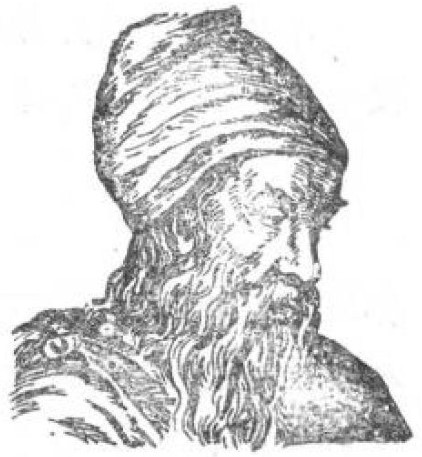
\includegraphics[width=4cm]{../pic/czwl1-ch6-archimedes}
    \caption*{阿基米德(公元前 287 ~ 212)}\label{fig:6-archimedes}
    \end{minipage}
    \qquad
    \begin{minipage}{10cm}
    \centering
    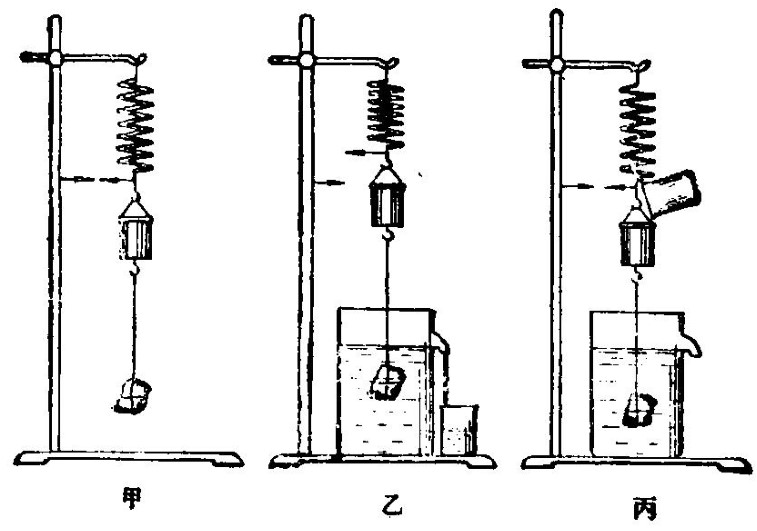
\includegraphics[width=9cm]{../pic/czwl1-ch6-3}
    \caption{阿基米德定律实验}\label{fig:6-3}
    \end{minipage}
\end{figure}

在弹簧下面挂一个金属筒,筒下面吊一个金属块,记下弹簧伸长后到达的位置(图 \ref{fig:6-3} 甲)。
另取一个水槽,槽里的水装到溢水管口。把金属块全部没入槽里水面下,金属块受到水的浮力,弹簧缩短。
被金属块排开的水从溢水管流到小杯里(图 \ref{fig:6-3} 乙)。
然后把小杯里的水全部倒进金属筒,这时弹簧又伸长到原来的位置(图 \ref{fig:6-3} 丙)。
这说明,\CJKunderwave{金属块所受的浮力,等于它排开的水重}。

在这个实验里如果金属块只有一部分浸在水里,实验表明,金属块受到的浮力仍等于它排开的水重。

不用水而用酒精或盐水等液体来做上面的实验,结果都一样。

所以,\textbf{浸在液体里的物体受到向上的浮力,浮力的大小等于物体排开的液体受到的重力}。
这就是\textbf{阿基米德定律}。

阿基米德定律,不仅适用于液体,也适用于气体。
\CJKunderwave{物体在气体中所受浮力的大小,等于被物体排开的气体受到的重力}。

\liti 体积是 $100\lflm$ 的铁块,重 7.6 牛顿。
当它全部浸没在水中时,受到多大的浮力?
这时候如果把铁块挂在弹簧秤上,弹簧秤的读数是多少?

铁块受到的浮力 $F_\text{浮}$ 可以用阿基米德定律求出,它等于铁块排开的水重 $G_\text{水}$。
由于铁块全部浸没在水中,所以铁块排开的水的体积 $V_\text{排}$ 就等于铁块的体积 $100\lflm = 0.0\;001\lfm$。
铁块浸没在水中时,弹簧秤的读数 $F$ 等于铁块重 $G_\text{铁}$ 减去水对铁块的浮力 $F_\text{浮}$。

解:$\begin{aligned}[t]
    F_\text{浮} &= G_\text{水} = \rho_\text{水} gV_\text{排} \\
        &= 1000 \qkmlfm \times 9.8 \ndmqk \times 0.0\;001 \lfm \\
        &= 0.98\niudun \;\juhao
\end{aligned}$

$F = G_\text{铁} - F_\text{浮} = 7.6 \niudun - 0.98 \niudun \approx 6.6 \niudun$。

答:铁块受到的浮力为 0.98 牛顿,这时弹簧秤的读数为 6.6 牛顿。



\nonumsection{阅读材料:阿基米德的故事}

二千多年前,在意大利西西里岛上曾经有一个叙拉古王国,阿基米德是这个王国的国王希罗的亲戚。
有一回,国王希罗找了一个珠宝商,给了他一些金子,要珠宝商制作一顶美丽的王冠。
不久,王冠做成了,非常精致漂亮,也跟原来给的黄金一样重,国王很喜欢。
但是希罗疑心王冠不是纯金的,他怀疑珠宝商盗窃了他的一部分黄金,在王冠中掺进了同样重的白银。
于是国王便把学者阿基米德请来,请他鉴定王冠是不是纯金的,但是不准把王冠弄坏了。

阿基米德冥思苦想,研究了许多天,还是没有结果。但是他没有灰心,仍然继续思索。
一天早上,阿基米德到浴室里去洗澡,浴缸里盛满了水,当他跨入浴缸时,他注意到水面上升并且从浴缸里往外溢,水被他的身体排开了。
这一下,日夜苦思的阿基米德顿时豁然开朗,急忙跳出浴缸,兴奋地边跑边喊:“我找到了!我找到了!” 往家里奔去。

阿基米德找到了解决王冠问题的方法。把王冠浸没在水中,根据它排开的水的体积可以知道王冠的体积。
因为白银的密度比黄金的密度小,所以如果王冠中掺进了白银,王冠的体积就会大于同样重的黄金的体积。


\lianxi

(1) 图 \ref{fig:6-4} 中,$A$,$B$ 两块金属的体积相等,哪个受到的浮力大?

\begin{figure}[htbp]
    \centering
    \begin{minipage}{5cm}
    \centering
    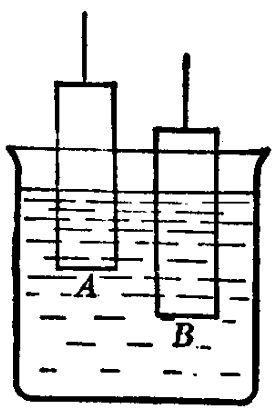
\includegraphics[width=4cm]{../pic/czwl1-ch6-4}
    \caption{}\label{fig:6-4}
    \end{minipage}
    \qquad
    \begin{minipage}{9cm}
    \centering
    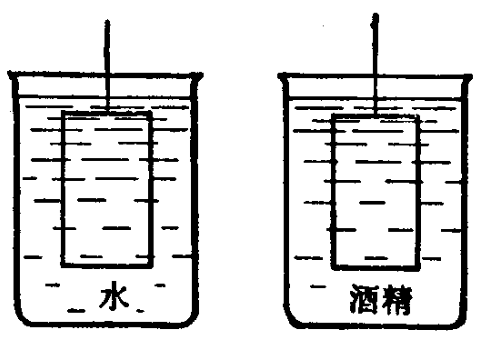
\includegraphics[width=8cm]{../pic/czwl1-ch6-5}
    \caption{}\label{fig:6-5}
    \end{minipage}
\end{figure}

(2) 图 \ref{fig:6-5} 中,两个容器中金属块的体积相等,哪个受到的浮力大?

(3) 物体浸没在液体中,在不同深度受到的浮力是否相等?为什么?设计一个实验来验证你的答案是否正确。

(4) 体积是 $50\lflm$ 的玻璃塞子,浸没在煤油里,煤油对它的浮力有多大?

(5) 有一个体积是 $1500\lfm$ 的气球,在地面附近空气对它的浮力是多大?

(6) 质量为 234 克的钢块,它的体积是多大?把它浸没在水中,受到的浮力是多大?

(7) 如果图 \ref{fig:6-2} 中的正方体的边长为 10 厘米,上表面离水面 5 厘米,上、下表面受到的压力差是多少?
这个物体排开的水重是多少?比较用这两种方法求得的浮力是否相等。


